\documentclass[12pt]{article}

\usepackage{amsmath,amsfonts,amsthm,amssymb}
\usepackage{color}
\usepackage{graphicx}
\usepackage{wrapfig}
\usepackage{epsfig}
%\usepackage{subfigure}
\usepackage{times}
\usepackage{xspace}
\usepackage{url}
\usepackage{pdfpages}
\usepackage{array}
\usepackage{subfig}
\usepackage{multirow}
\usepackage{dblfloatfix} 

\setlength{\topmargin}{0.0in}     % top of paper to head (less one inch)
\setlength{\headheight}{0in}      % height of the head
\setlength{\headsep}{0in}         % head to the top of the body
\setlength{\textheight}{9.0in}    % height of the body
\setlength{\oddsidemargin}{-.25in} % left edge of paper to body (less one inch)
\setlength{\evensidemargin}{0mm}  % ditto, even pages
\setlength{\textwidth}{7.0in}     % width of body
\setlength{\topskip}{0in}         % top of body to bottom of first line of text
\setlength{\parindent}{1pc}       

\begin{document}
\thispagestyle{empty}
%%%%%%%%%%%%%%%%%%%%%%%%%%%%%%%%%%%%%%%%%%%%%%%%%%%%%%%%%%%%%%%%%%%%%%%%%%%%%%%%%%%%%%%%
% Project Summary
%%%%%%%%%%%%%%%%%%%%%%%%%%%%%%%%%%%%%%%%%%%%%%%%%%%%%%%%%%%%%%%%%%%%%%%%%%%%%%%%%%%%%%%%
\begin{center}
{\Large\bf Assignment \#6: StreamGraphs}
\vspace{3mm}
\\Caitlin Ross \& Noah Wolfe
\\03/21/2016
\\*[3mm]
\end{center}
%%%%%%%%%%%%%%%%%%%%%%%%%%%%%%%%%%%%%%%%%%%%%%%%%%%%%%%%%%%%%%%%%%%%%%%%%%%%%%%%%%%%%%%%
% Task Objects
%%%%%%%%%%%%%%%%%%%%%%%%%%%%%%%%%%%%%%%%%%%%%%%%%%%%%%%%%%%%%%%%%%%%%%%%%%%%%%%%%%%%%%%%
\section{Data Source (ROSS)}
%Description of the data source and corresponding applications.
In this assignment, we have decided to generate/collect data from our ROSS research projects. 
ROSS is a massively parallel discrete-event simulator that
can process billions of events per second \cite{Holder}, \cite{Bauer}. ROSS
models are made up of a collection of logical processes (LPs).
Each LP models a distinct component of the system. LPs
interact with one another through events in the form of time-stamped messages. An MPI task is abstracted as a processor
element (PE) in ROSS. Each PE owns a number of LPs and
schedules events in time-stamp order for all LPs assigned to
it. Events that are destined for a logical process on another
PE (i.e. remote events) are sent as MPI messages. 

For this assignment we decided to collect remote event data for each PE in the simulation. Running with 8 total PE's we collect the total number of MPI messages sent per PE at each instance of simulation time. The first dataset is generated with a simulation using the Dragonfly network interconnect model with uniform random traffic using minimal routing. The second dataset is generated using a Slim Fly network interconnect model simulation also using uniform random traffic and minimal routing. The data is extracted into a simple csv format with the following layout: PE\#, sim-time, remote-events. We started off collecting 1,000 points in time for each PE but the resulting streamgraphs looked terrible (very discrete and spiky instead of smooth and continuous) so we dropped the number of time samples down to 100 per PE for a total of 800 points in time per graph.

\section{Bar Graph Visualization} \label{bar}
In order to generate the stacked bar graphs, we decided to use Excel. Excel is very straightforward and has a simple interface with many options for color. Also, our data set was in the csv format so loading into Excel was very easy. The resulting stacked bar graphs are shown in Figure \ref{Bar}. Presenting the data in bar graph form leaves a lot to be desired. On the positive side, one can quickly glean the overall trend of all MPI sends for all PEs in each simulation but that is it. The separation and differences between the different PEs is very difficult to see which is a direct result of trying to smash so much data into bars in a small horizontal area. It forces the width of the bars to be very small. Also, as a result of the small bar widths, color isn't allowed to have a beneficial effect on the data visualization. One of the strong properties of Excel is selection of color schemes but unfortunately the bar graph cancels out the color capability.
\begin{figure}[!ht]
     \centering
     \subfloat[][Slim Fly]{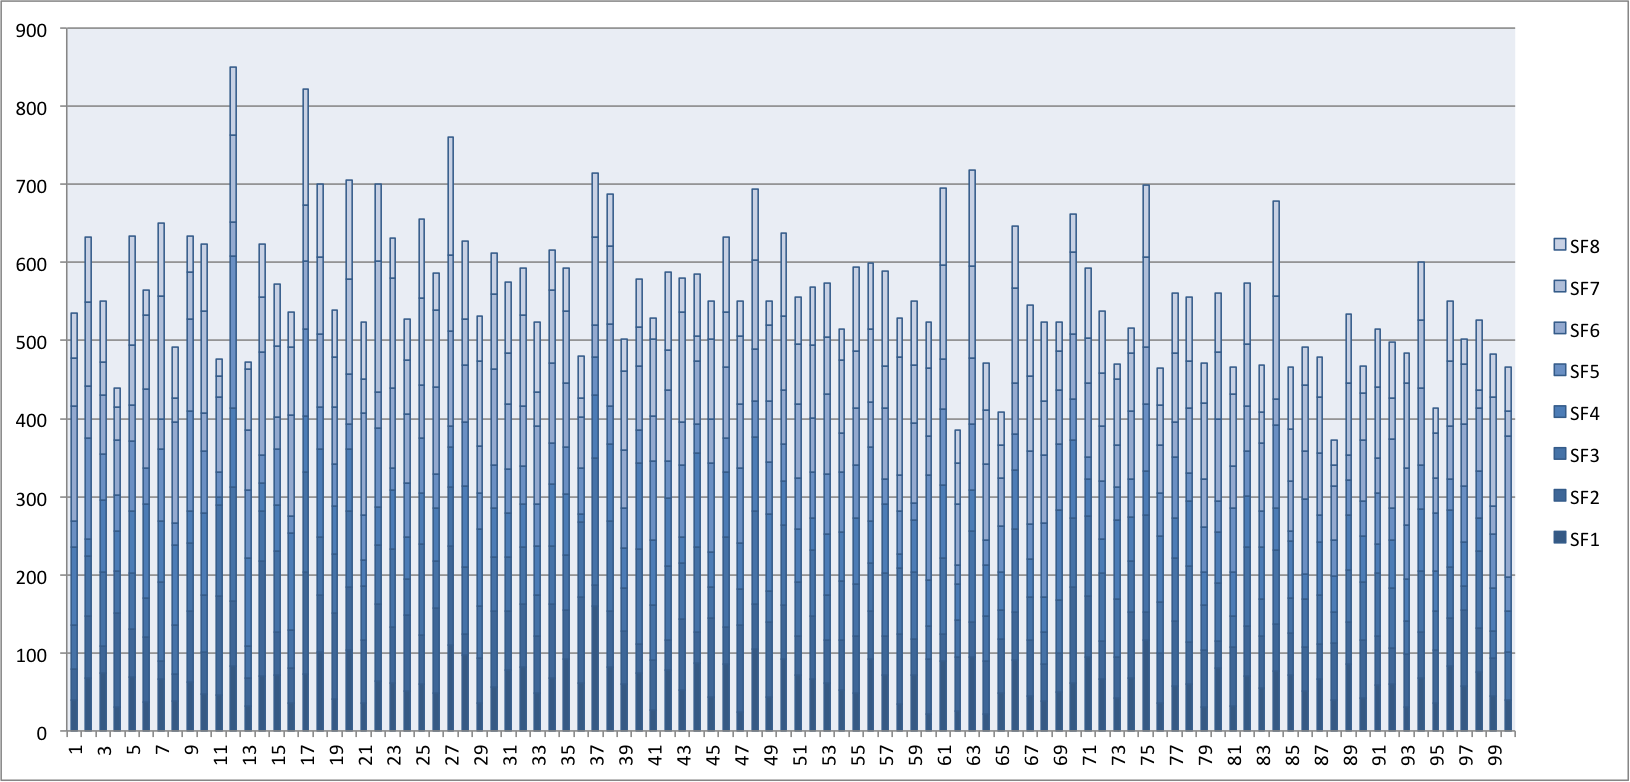
\epsfig{file=figures/slimfly-bar.png, height=3.5in, width=6.50in}\label{top}}\\
     \subfloat[][Dragonfly]{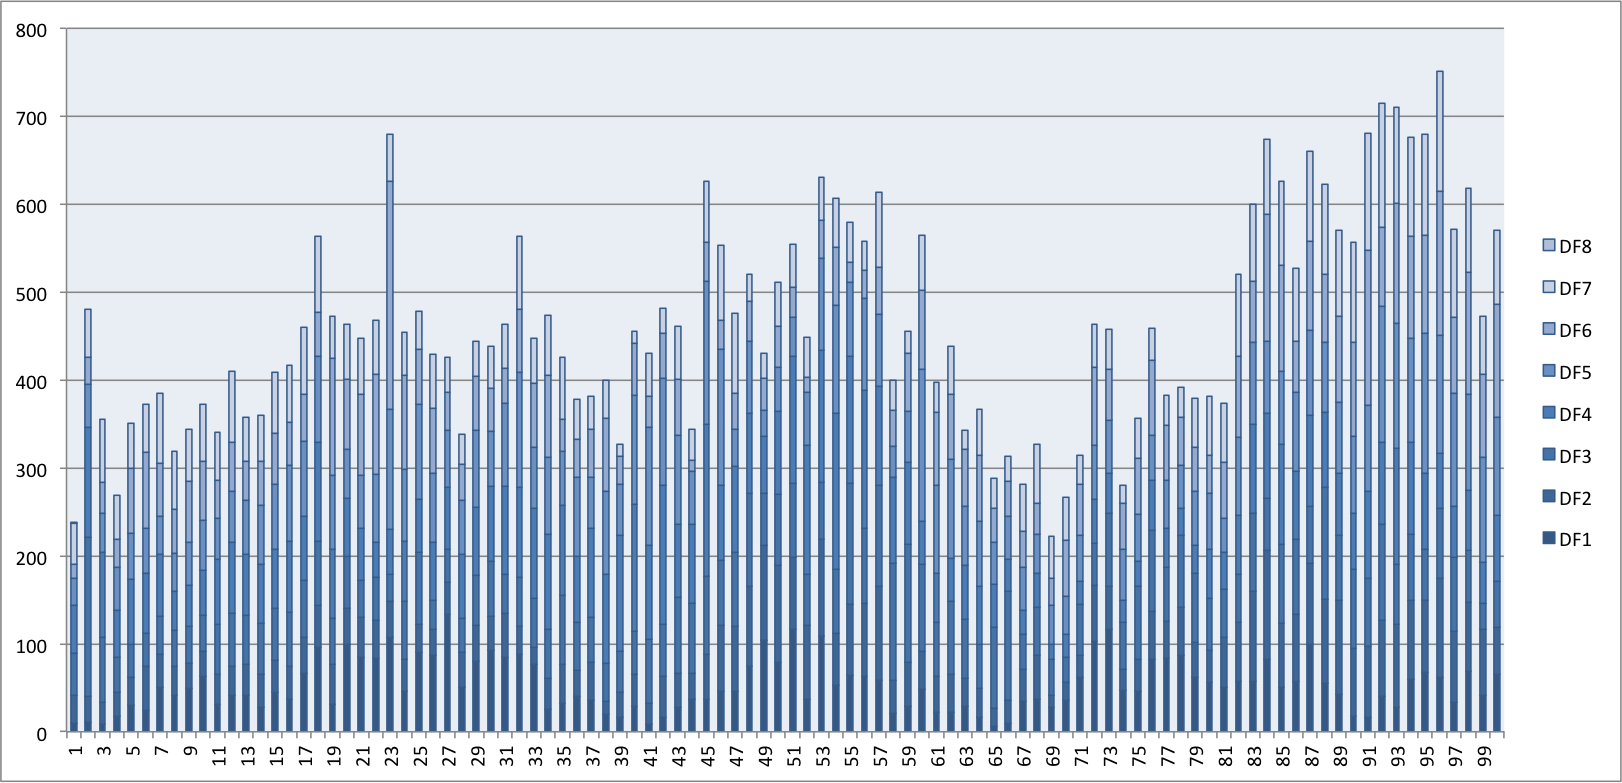
\epsfig{file=figures/dragonfly-bar.png, height=3.5in, width=6.50in}\label{bot}}
     \caption{Stacked bar chart visualizations of the Dragonfly and Slim Fly remote message simulation data sets showing the number of MPI messages being sent from each PE in the simulation over time. Both figures start with PE 1 ("SF1" or "DF1" in the legends) on the bottom of the stacked bars and the data for the following PEs is stacked on top, in order, and finishing with PE 8 ("SF8" or "DF8" in the legends) on top. Each bar along the x-axis represents a different point in the simulation time.}
     \label{Bar}
\end{figure}

\section{Stream Graph Visualization} \label{stream}

\begin{figure}[!ht]
     \centering
     \subfloat[][Slim Fly]{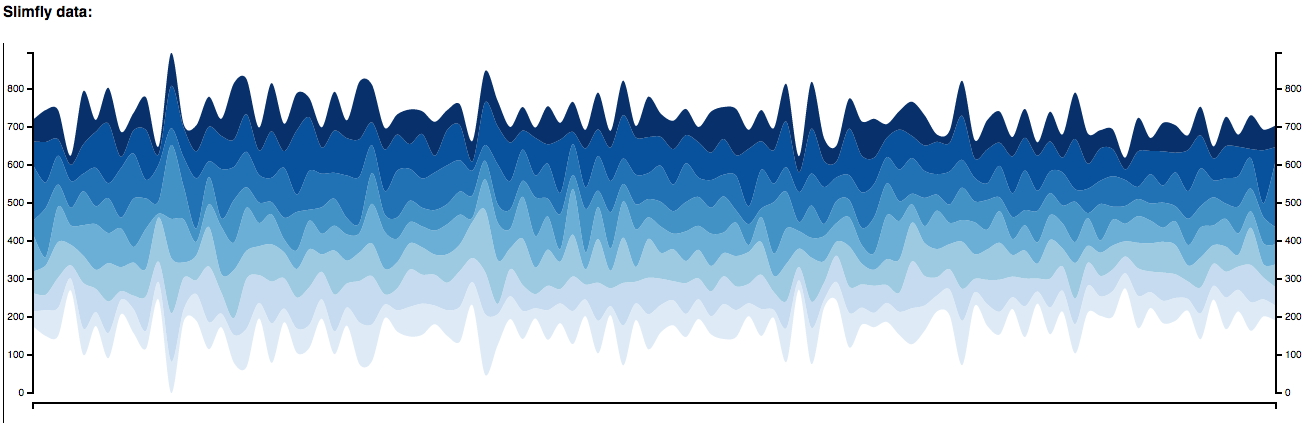
\epsfig{file=figures/slimfly-sg.png, height=2.5in, width=6.50in}\label{top-stream}}\\
     \subfloat[][Dragonfly]{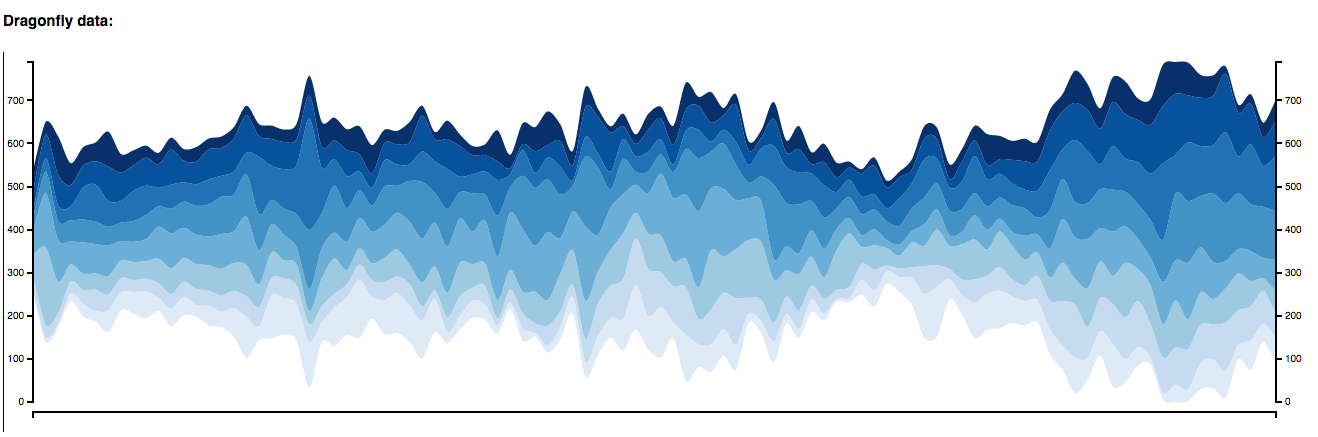
\epsfig{file=figures/dragonfly-sg.png, height=2.5in, width=6.50in}\label{bot-stream}}
     \caption{Stream graph visualizations of the Dragonfly and Slim Fly remote message simulation data sets showing the number of MPI messages being sent from each PE in the simulation over time. Both figures start with PE 1 (lightest blue) on the bottom with the following PEs layered in order on top, and finishing with PE 8 (darkest blue) on top. The x-axis shows simulation time increasing from left to right.  The vertical height of a layer (i.e., PE) corresponds to the number of remote events for that PE.}
     \label{sg}
\end{figure}

We used William Turman's Stream graph D3 implementation \cite{Stream} to create the stream graphs of our data.  This required very little modification to work.  We got our data into a similar format as the example, except that we use an integer to represent simulated time, instead of using a real date as the example does.  We had to make some Javascript modifications to appropriately handle the time information.  Then we were able to add both data sets to the same page.   The stream graphs of both the Slimfly and Dragonfly data are shown in Figure~\ref{sg}.  The colors used are from the ColorBrewer website~\cite{Colorbrewer}.

The graphs are hosted at \url{https://caitlinross.github.io/vis/streamgraph.html}.  There is an interactive aspect that is not shown in the figures.  When hovering over a layer, several things occur.  The opacity of the other layers are decreased to make the layer selected stand out.  A vertical bar moves to where the mouse pointer is.  Finally, a tooltip appears that shows the PE id and the value for that PE at that point in time.


\section{Bar vs Stream Graph Comparison}
%Analyze the effectiveness of the bar graph vs. streamgraph in showing off the differences and similarities in the two datasets. How well do these plots allow the viewer to make accurate conclusions about the data?
Overall, we think it is clear the stream graph is a much better choice for large time-series data sets as compared with stacked bar graphs. Both graph approaches make observation and analysis of global/general features quick and easy. After a quick glance at both sets of visualizations, it is clear the Slim Fly network has a much more consistent MPI send rate while the Dragonfly is more sporadic. However, the similarities between the bar graphs and stream graphs end there. On one hand, the stream graph visualizations perform better in representing the differences in the PEs, clearly showing the separation of the PE data by colors and making it easy to follow along the x-axis. With the bar charts, it's nearly impossible to differentiate between the different PEs and the thin bars makes it impossible for any coloring to help the matter as there is no space to color. On the other hand, the labels on the y-axis don't make much sense in the stream graph, since the baseline is not set to 0. The stacked bar graph chart has a very clear y-axis and thus makes it easier to see the number of remote events for all PEs for a given point in simulated time. These numbers can of course be calculated from the stream graph y-axis with some extra effort. In the end, the stream graph does a much better job of providing detailed analysis when dealing with large amounts of data as shown in this report. The ability to distinguish and follow trends in the data at the global simulation and local PE levels makes the stream graph the preferred choice.
 
% Bibliography
\bibliographystyle{abbrv}
\bibliography{HW4}

\end{document}


%\begin{figure}[!ht]
%     \centering
%     \subfloat[][twopi]{\epsfig{file=figures/MMS7-3-17.png, height=2.2in, width=4.80in}\label{vis-100-1}}\\
%     \subfloat[][dot]{\epsfig{file=figures/MMS7-3-12.png, height=2.0in, width=3.00in}\label{vis-100-2}}
%     \subfloat[][circo]{\epsfig{file=figures/MMS7-3-circo.png, height=2.0in, width=3.0in}\label{vis-100-3}}\\
%     \caption{Visualizations of the class social network data using a collection of Graphviz graph drawing programs. Red lines represent "before RPI" connections, blue represent "lived with" connections and black represent "Data Structures" connections. }
%     \label{vc-occupancy}
%\end{figure}

%\begin{figure}[!h]
%\centering
%\epsfig{file=figures/storyboard.jpg, width=5.5in}
%\caption{Storyboard showing the desired layout and interaction of the network visualization tool in D3.}
%\label{good}
%\end{figure}